\def\year{2022}\relax
%File: formatting-instructions-latex-2022.tex
%release 2022.1
\documentclass[letterpaper]{article} % DO NOT CHANGE THIS
\usepackage[submission]{aaai23}  % DO NOT CHANGE THIS
\usepackage{times}  % DO NOT CHANGE THIS
\usepackage{helvet}  % DO NOT CHANGE THIS
\usepackage{courier}  % DO NOT CHANGE THIS
\usepackage[hyphens]{url}  % DO NOT CHANGE THIS
\usepackage{graphicx} % DO NOT CHANGE THIS
\urlstyle{rm} % DO NOT CHANGE THIS
\def\UrlFont{\rm}  % DO NOT CHANGE THIS
\usepackage{natbib}  % DO NOT CHANGE THIS AND DO NOT ADD ANY OPTIONS TO IT
\usepackage{caption} % DO NOT CHANGE THIS AND DO NOT ADD ANY OPTIONS TO IT
\DeclareCaptionStyle{ruled}{labelfont=normalfont,labelsep=colon,strut=off} % DO NOT CHANGE THIS
\frenchspacing  % DO NOT CHANGE THIS
\setlength{\pdfpagewidth}{8.5in}  % DO NOT CHANGE THIS
\setlength{\pdfpageheight}{11in}  % DO NOT CHANGE THIS
%
% These are recommended to typeset algorithms but not required. See the subsubsection on algorithms. Remove them if you don't have algorithms in your paper.
% \usepackage{algorithm}
% \usepackage{algorithmic}
% \usepackage[noend]{algpseudocode}

%
% These are are recommended to typeset listings but not required. See the subsubsection on listing. Remove this block if you don't have listings in your paper.
\usepackage{newfloat}
\usepackage{listings}
\lstset{%
	basicstyle={\footnotesize\ttfamily},% footnotesize acceptable for monospace
	numbers=left,numberstyle=\footnotesize,xleftmargin=2em,% show line numbers, remove this entire line if you don't want the numbers.
	aboveskip=0pt,belowskip=0pt,%
	showstringspaces=false,tabsize=2,breaklines=true}
%\floatstyle{ruled}
%\newfloat{listing}{tb}{lst}{}
%\floatname{listing}{Listing}

%
% user import packages
\usepackage{amsfonts}
\usepackage{amsthm}
\usepackage{amsmath}
\usepackage{paralist}
\usepackage{todonotes}
\usepackage{booktabs}
\usepackage{varwidth}
\usepackage{algorithm}
\usepackage[noend]{algpseudocode}
\usepackage{xcolor}
\usepackage{booktabs} 
% \usepackage[ruled, noend, linesnumbered]{algorithm2e}  
\usepackage{csquotes}
\usepackage{subcaption}
\usepackage{amssymb} 
\usepackage{mathbbol}
\usepackage{tikz}
\usetikzlibrary{aiplans}


\scheme{SinglePrec}{0}{
	text = {\textbf{A}},
	pre  = {a}
}

\scheme{SingleAdd}{0}{
	text = {\textbf{B}},
	effs = { a}
}

\scheme{SingleDelete}{0}{
	text = {\textbf{C}},
	effs = { {{$\neg$}a} }
}


\scheme{SinglePrecAlt}{0}{
	text = {\textbf{D}},
	pre  = {a}
}

\scheme{SingleAddAlt}{0}{
	text = {\textbf{E}},
	effs = { a}
} 

\scheme{PrimitiveA}{0}{
	text = {\textbf{A}},
	pre  = {a},
	effs = { {{$\neg$}a}, {b} }
}

\scheme{PrimitiveB}{0}{
	text = {\textbf{B}},
	pre = {b},
	effs = {{{$\neg$}b}, {c}}
}

\scheme{PrimitiveC}{0}{
	text = {\textbf{C}},
	pre = {c},
	eff = {{$\neg$}c}
}

\nocopyright
%
% PDF Info Is REQUIRED.
% For /Title, write your title in Mixed Case.
% Don't use accents or commands. Retain the parentheses.
% For /Author, add all authors within the parentheses,
% separated by commas. No accents, special characters
% or commands are allowed.
% Keep the /TemplateVersion tag as is
\pdfinfo{
/Title (ORdering is half the battle -- Establishing Totally Ordered HTN
Planning Problems is Half the Job (to Getting them Solved More Efficiently))
%/Title (Ordnung ist das halbe Leben -- Establishing Totally Ordered HTN
%Planning Problems is Half the Job (to Getting them Solved More Efficiently))
/Author (Anonymous)
/TemplateVersion (2022.1)
}

% DISALLOWED PACKAGES
% \usepackage{authblk} -- This package is specifically forbidden
% \usepackage{balance} -- This package is specifically forbidden
% \usepackage{color (if used in text)
% \usepackage{CJK} -- This package is specifically forbidden
% \usepackage{float} -- This package is specifically forbidden
% \usepackage{flushend} -- This package is specifically forbidden
% \usepackage{fontenc} -- This package is specifically forbidden
% \usepackage{fullpage} -- This package is specifically forbidden
% \usepackage{geometry} -- This package is specifically forbidden
% \usepackage{grffile} -- This package is specifically forbidden
% \usepackage{hyperref} -- This package is specifically forbidden
% \usepackage{navigator} -- This package is specifically forbidden
% (or any other package that embeds links such as navigator or hyperref)
% \indentfirst} -- This package is specifically forbidden
% \layout} -- This package is specifically forbidden
% \multicol} -- This package is specifically forbidden
% \nameref} -- This package is specifically forbidden
% \usepackage{savetrees} -- This package is specifically forbidden
% \usepackage{setspace} -- This package is specifically forbidden
% \usepackage{stfloats} -- This package is specifically forbidden
% \usepackage{tabu} -- This package is specifically forbidden
% \usepackage{titlesec} -- This package is specifically forbidden
% \usepackage{tocbibind} -- This package is specifically forbidden
% \usepackage{ulem} -- This package is specifically forbidden
% \usepackage{wrapfig} -- This package is specifically forbidden
% DISALLOWED COMMANDS
% \nocopyright -- Your paper will not be published if you use this command
% \addtolength -- This command may not be used
% \balance -- This command may not be used
% \baselinestretch -- Your paper will not be published if you use this command
% \clearpage -- No page breaks of any kind may be used for the final version of your paper
% \columnsep -- This command may not be used
% \newpage -- No page breaks of any kind may be used for the final version of your paper
% \pagebreak -- No page breaks of any kind may be used for the final version of your paperr
% \pagestyle -- This command may not be used
% \tiny -- This is not an acceptable font size.
% \vspace{- -- No negative value may be used in proximity of a caption, figure, table, section, subsection, subsubsection, or reference
% \vskip{- -- No negative value may be used to alter spacing above or below a caption, figure, table, section, subsection, subsubsection, or reference

\setcounter{secnumdepth}{0} %May be changed to 1 or 2 if section numbers are desired.

% The file aaai22.sty is the style file for AAAI Press
% proceedings, working notes, and technical reports.
%

% Title

% Your title must be in mixed case, not sentence case.
% That means all verbs (including short verbs like be, is, using,and go),
% nouns, adverbs, adjectives should be capitalized, including both words in hyphenated terms, while
% articles, conjunctions, and prepositions are lower case unless they
% directly follow a colon or long dash

%Example, Single Author, ->> remove \iffalse,\fi and place them surrounding AAAI title to use it
% \iffalse


\newtheorem{theorem}{Theorem} 

\newcommand{\Eff} {\ensuremath{\mathit{eff}}}  % example command without arguments
\newcommand{\Pre} {\ensuremath{\mathit{pre}}}  % (again)

\newcommand{\Add} {\ensuremath{\mathit{add}}}
\newcommand{\Del} {\ensuremath{\mathit{del}}}
\newcommand{\PreS} {\ensuremath{\mathit{pre^{*}}}}
\newcommand{\AddS} {\ensuremath{\mathit{add^{*}}}}
\newcommand{\DelS} {\ensuremath{\mathit{del^{*}}}}
\newcommand{\singlePrec} {\ensuremath{\mathit{ \mathord{\prec} }}}
\newcommand{\tasks} {\ensuremath{\mathit{tasks}}}

%\newcommand{\EffPlus} {\ensuremath{\mathit{eff^{+}_{*}}}}
%\newcommand{\EffMinus} {\ensuremath{\mathit{eff^{-}_{*}}}}
\newcommand{\PossEffPlus} {\ensuremath{\mathit{\textit{poss-eff}^{+}_{*}}}}
\newcommand{\PossEffMinus} {\ensuremath{\mathit{\textit{poss-eff}^{-}_{*}}}}

%\newcommand{\RelEffPlus} {\ensuremath{\mathit{\textit{eff}^{\emptyset +}_{*}}}}
%\newcommand{\RelEffMinus} {\ensuremath{\mathit{\textit{eff}^{\emptyset -}_{*}}}}
\newcommand{\RelPossEffPlus} {\ensuremath{\mathit{\textit{poss-eff}^{\emptyset +}_{*}}}}
\newcommand{\RelPossEffMinus} {\ensuremath{\mathit{\textit{poss-eff}^{\emptyset -}_{*}}}}


\author {
    Submission
}
\affiliations{
    Anonymous
}
% \fi


%Example, Multiple Authors, ->> remove \iffalse,\fi and place them surrounding AAAI title to use it
\iffalse 
%\title{Ordnung ist das halbe Leben -- Establishing Totally Ordered HTN
%	Planning Problems is Half the Job (to Getting them Solved More Efficiently)}
\author {
    % Authors
    Anonymous

}
\affiliations {
    % Affiliations
    Anonymous
}
\fi

\title{``Order is Half of Life'' -- Establishing Totally Ordered HTN Planning Problems is Half the Job (to Getting them Solved Efficiently)}

%\title{Ordnung ist das halbe Leben -- Establishing Totally Ordered HTN
%	Planning Problems is Half the Job (to Getting them Solved More Efficiently)}


% REMOVE THIS: bibentry
% This is only needed to show inline citations in the guidelines document. You should not need it and can safely delete it.
% \usepackage{bibentry}
% END REMOVE bibentry

\begin{document}
% citiation commands
\newcommand{\shortCite}[1] {\citeauthor{#1} (\citeyear{#1})}

% symbols
\newcommand{\groundProb}{\ensuremath{\Pi}}
\newcommand{\lit}{\ensuremath{\mathcal{F}}}
\newcommand{\cTasks}{\ensuremath{\mathcal{C}}}
\newcommand{\pTasks}{\ensuremath{\mathcal{A}}}
\newcommand{\methods}{\ensuremath{\mathcal{M}}}
\newcommand{\domain}{\ensuremath{\mathcal{D}}}
\newcommand{\eff}{\ensuremath{\mathit{eff}}}
\newcommand{\effPos}[1]{\ensuremath{\eff{}^{+}(#1)}}
\newcommand{\effNeg}[1]{\ensuremath{\eff{}^{-}(#1)}}
\newcommand{\preCond}[1]{\ensuremath{\mathit{prec}(#1)}}
\newcommand{\effPosExt}[1]{\ensuremath{\mathtt{eff}^{+}(#1)}}
\newcommand{\effNegExt}[1]{\ensuremath{\mathtt{eff}^{-}(#1)}}
\newcommand{\preCondExt}[1]{\ensuremath{\mathtt{prec}(#1)}}
\newcommand{\parOrd}{\ensuremath{\mathord{\prec}}}
\newcommand{\seqSet}[1]{\ensuremath{\mathcal{L}(#1)}}

% math notations
\newcommand{\NP}{\ensuremath{\mathbb{NP}}}
\newcommand{\PTIME}{\ensuremath{\mathbb{P}}}
\newcommand{\EXPTIME}{\ensuremath{\mathbb{EXPTIME}}}
\newcommand{\powerSet}[1]{\ensuremath{2^{#1}}}
\maketitle

\begin{abstract} 
HTN planning is in general undecidable, yet there exist efficient
planning algorithms. An important subclass is that of totally ordered
HTN planning problems. Not only is this class decidable, but also easier
to handle algorithmically since tasks cannot interleave anymore.
Consequently, several specialized solvers exist, and dedicated tracks at
the International Planning Competition (IPC) in both 2020 and 2023. We
were able to show that almost all currently existing partially ordered
planning benchmarks can be turned into totally ordered ones without
sacrificing solvability. Establishing totally ordered problems in a
preprocessing technique thus allows to use planning systems, heuristics,
pruning techniques (etc.) that are only available for totally ordered
problems. This allows solving problems more efficiently and with
better-informed techniques, at the (little) cost of doing a
preprocessing technique. We show that in only a very few cases
linearization isn't possible, and in all others establishing a total
order pays off \emph{significantly}, thus establishing our technique as
a significant ingredient in the state of the art for solving partially
ordered HTN problems. As a side contribution, we identify a new class of
decidable (EXPTIME-complete) HTN problems, namely those where our
preprocessing technique is guaranteed to be solvability-preserving.
\end{abstract}
 
 

 
 
 
\section{Introduction}
% Hierarchical Task Network (HTN) planning, as described by \shortCite{HTNSurvey}, is a hierarchical approach to planning where so-called \emph{compound tasks} are kept being refined until primitive ones (also called \emph{actions}) are obtained which form a \emph{plan}. Research on HTN planning has drawn increasing interests in the last decade due to its expressive power. More concretely, HTN planning can simulate the classes of formal languages ranging from star-free languages to (a strict subset of) context-sensitive languages, whereas non-hierarchical (i.e., classical) planning can only express a strict subset of star-free languages \cite{Hoeller2016Expressivity,Lin2022LTLExpressivity}. % As defined by \cite{HTNSurvey},  %  and \cite{IntroGhallab},
% tasks in HTN planning are either primitive, corresponding to an action that can be taken, or compound. HTN problems have a set of methods that specify how one might achieve a given compound task, by decomposing it into a set of sub-tasks. A compound task may even decompose into itself, either directly via a method, or indirectly via a sequence of method applications. If decomposition leads to a sequence of primitive tasks executable from the initial state, then this sequence of actions is a solution to the problem, also known as a \enquote{plan}. 

One major problem faced by the HTN planning community is the high computational complexity of HTN planning problems. Specifically, \shortCite{Erol1996HTNComplexity} have shown that an HTN planning problem is undecidable in general, and thus, finding a solution to an HTN problem is still a challenge task even for the state-of-the-art HTN planner.

In this paper, we propose a novel approach which transforms a general HTN planning problem (where a compound task is refined into a \emph{partially ordered} set of subtasks) into a \emph{totally ordered} one which is a special form of HTN planning problems and in which a compound task can only be refined into a \emph{sequence} (i.e., a totally ordered set) of subtasks. More importantly, our approach assures that any solution to the transformed problem is also a solution to the original problem, and our approach works for both the grounded and the lifted formalism. Thus, by employing this approach (e.g., as a preprocessor), we could reduce the complexity of finding a solution to the original problem because, as proved by \shortCite{Alford2015TightHTNBounds}, it is \EXPTIME{}-complete to solve a totally ordered HTN planning problem, and specialized HTN planning techniques (e.g., heuristics and pruning techniques) for only totally ordered problems can also be deployed for solving the transformed problem.

Notably, our approach does \emph{not} guarantee that at least one solution will be preserved after the transformation. However, our empirical evaluation shown that it is rarely the case that none solutions are preserved. More specifically, there is only one domain in our benchmark set where problems become unsolvable after the transformation. Additionally, we will also present certain criteria which assert that at least one solution will be preserved if they are satisfied.

As a side contribution, our approach can also be exploited to create new total order HTN planning domains from partial order ones. This might be particularly useful by taking into account the upcoming 2023 International Planning Competition (IPC) on HTN planning.


% In totally ordered HTN planning, or TOHTN planning, methods specify a total order on the sub-tasks. In partially ordered HTN planning, or POHTN planning, methods might only specify a partial order on the sub-tasks. 

% % Certain kinds of problems might be naturally more suited to being modelled as a partially ordered problem, for example, the actions \enquote{deliver package 1 to city A} and \enquote{deliver package 2 to city B} -- these are essentially unrelated goals in a real transport scenario, and so modelling the problem to require that one task be completed before the other would be unnecessarily limiting the possible solution space. For some problems, such over-specification may remove all valid solutions. 

% Many problems might be naturally more suited to being modelled as POHTN problems. However, for \emph{solving} the problem, it is desirable to have additional constraints that reduces the search space, while still preserving at least some of the actual solutions. For example, \cite{ErolHTNExpressivity} proved that POHTN planning is expressive enough to model undecidable problems, such as the language intersection problem of two context-free languages. On the other hand, TOHTN planning is not expressive enough to model undecideable problems. Where this is possible, it results in lower worst-case solving time. Converting the problem to a TOHTN problem allows us to exploit that fact to solve the problem more quickly.

% Another benefit of transforming a POHTN problem to a TOHTN problem is that the additional structure to the problem could allow us to deploy specialised algorithms and heuristics for the totally ordered case. % Also, heuristic design is comparably easy for total-order problems due to the missing interaction between tasks.
% The drawback to this approach is that, due to the greater expressivity of POHTN planning, there may exist POHTN problems that cannot be solved when converted to a TOHTN problem. 
% Fortunately, not every POHTN problem is guaranteed to be undecidable, and so could still be transformed while preserving at least one solution. In fact, the state-of-the-art panda$_\pi$ planner and \cite{HTN2SAS} both use a compilation to classical planning, another decidable planning class.
% In this paper we present and investigate an algorithm for converting POHTN problems to TOHTN problems. We prove that when certain criteria are met, it guarantees that at least one solution will be preserved. 
% Also, we obtain a new class of decidable problems, namely those that satisfy the above mentioned criterion. Finally, we show that, even when these criteria are not met, very few problems are rendered unsolvable by the transformation, and that it greatly reduces solving time for problems, with gains being bigger for more difficult problems. 
Hierarchical Task Network (HTN) planning is a hierarchical approach to planning. As defined by \cite{HTNSurvey},  %  and \cite{IntroGhallab},
tasks in HTN planning are either primitive, corresponding to an action that can be taken, or compound. HTN problems have a set of methods that specify how one might achieve a given compound task, by decomposing it into a set of sub-tasks. A compound task may even decompose into itself, either directly via a method, or indirectly via a sequence of method applications. If decomposition leads to a sequence of primitive tasks executable from the initial state, then this sequence of actions is a solution to the problem, also known as a \enquote{plan}. 

In totally ordered HTN planning, or TOHTN planning, methods specify a total order on the sub-tasks. In partially ordered HTN planning, or POHTN planning, methods might only specify a partial order on the sub-tasks. 

% Certain kinds of problems might be naturally more suited to being modelled as a partially ordered problem, for example, the actions \enquote{deliver package 1 to city A} and \enquote{deliver package 2 to city B} -- these are essentially unrelated goals in a real transport scenario, and so modelling the problem to require that one task be completed before the other would be unnecessarily limiting the possible solution space. For some problems, such over-specification may remove all valid solutions. 

Many problems might be naturally more suited to being modelled as POHTN problems. However, for \emph{solving} the problem, it is desirable to have additional constraints that reduces the search space, while still preserving at least some of the actual solutions. For example, \cite{ErolHTNExpressivity} proved that POHTN planning is expressive enough to model undecidable problems, such as the language intersection problem of two context-free languages. On the other hand, TOHTN planning is not expressive enough to model undecideable problems. Where this is possible, it results in lower worst-case solving time. Converting the problem to a TOHTN problem allows us to exploit that fact to solve the problem more quickly.

Another benefit of transforming a POHTN problem to a TOHTN problem is that the additional structure to the problem could allow us to deploy specialised algorithms and heuristics for the totally ordered case. % Also, heuristic design is comparably easy for total-order problems due to the missing interaction between tasks.
The drawback to this approach is that, due to the greater expressivity of POHTN planning, there may exist POHTN problems that cannot be solved when converted to a TOHTN problem. 
Fortunately, not every POHTN problem is guaranteed to be undecidable, and so could still be transformed while preserving at least one solution.
In this paper we present and investigate an algorithm for converting POHTN problems to TOHTN problems. We prove that when certain criteria are met, it guarantees that at least one solution will be preserved. 
Also, we obtain a new class of decidable problems, namely those that satisfy the above mentioned criterion. Finally, we show that, even when these criteria are not met, very few problems are rendered unsolvable by the transformation, and that it greatly reduces solving time for problems, with gains being bigger for more difficult problems. 

 


\section{Hierarchical Planning Formalism}
For the purpose of illustrating our approach, we first present the HTN planning formalism used throughout the paper, including the grounded one and the lifted one. % The grounded HTN formalism is based on the one by \shortCite{HTNSurvey}.

\paragraph{Grounded HTN Planning} The grounded HTN planning formalism presented is based on the one by \shortCite{HTNSurvey}. A grounded HTN planning problem is a tuple $\groundProb{} = (\domain{}, tn_{I}, s_{I})$ with $\domain{} = (\lit{}, \pTasks{}, \cTasks{}, \delta, \methods{})$ being its \emph{domain}. $\lit{}$ is a set of \emph{propositions}. $\pTasks{}$ and $\cTasks{}$ are the set of \emph{primitive tasks} (also called \emph{actions}) and of \emph{compound tasks}, respectively. $\delta: \pTasks{} \to \powerSet{\lit{}} \times \powerSet{\lit{}} \times \powerSet{\lit{}}$ is a function mapping each primitive task $a \in \pTasks{}$ to its \emph{precondition}, \emph{positive effects}, and \emph{negative effects}, written $\delta(a) = (\preCond{a}, \effPos{a}, \effNeg{a})$. In particular, applying an action $a$ in some \emph{state} $s \in \powerSet{\lit{}}$ will result in a new state $s'$ with $s' = (s \setminus \effNeg{a}) \cup \effPos{a}$, written $s \to_{a} s'$, and $a$ is said to be applicable in $s$ \emph{iff} $\preCond{a} \subseteq s$. Furthermore, we say that a state $s'$ is obtained from another one $s$ by applying an action sequence $\pi = \langle a_{1} \cdots a_{n} \rangle$ in $s$, written $s \to^{\ast}_{\pi} s'$, \emph{iff} there exists a state sequence $\langle s_{0} \cdots s_{n} \rangle$ such that $s = s_{0}$, $s' = s_{n}$, and for each $1 \leq i \leq n$, $a_{i}$ is applicable in the state $s_{i - 1}$ and $s_{i - 1} \to_{a_{i}} s_{i}$. 

Each compound task $c \in \cTasks{}$ is \emph{decomposed} (refined) into a \emph{task network} $tn$, which is essentially a partial order \emph{multiset} of tasks, by a \emph{method} $m = (c, tn)$. Formally speaking, a task network $tn$ is a triple $(T, \parOrd{}, \alpha)$ where $T$ is a set of identifier, $\parOrd{} \subseteq T \times T$ is a partial order defined over $T$, and $\alpha: T \to \pTasks{} \cup \cTasks{}$ is a function mapping each identifier to a task. $\methods{}$ in the domain is the set of methods. $tn_{I}$ and $s_{I} \in \powerSet{\lit{}}$ are the initial task network and the initial state, respectively.

%TODO: decomposition 

A \emph{solution} to an HTN planning problem is a sequence of actions $\pi = \langle a_{1} \cdots a_{n} \rangle$ such that $s_{I} \to^{\ast}_{\pi} s$ for some state $s$, and there exists a task network $tn = (T, \parOrd{}, \alpha)$ such that $tn_{I} \Rightarrow^{\ast}_{\overline{m}} tn$ for some method sequence $\overline{m}$, and $tn$ possesses a linearization $\langle t_{1} \cdots t_{n} \rangle$ with $\alpha(t_{i}) = a_{i}$ for each $1 \leq i \leq n$. A linearization of $tn$ is a total order of $T$ that respects $\parOrd{}$.

As a special case of 

\section{Linearizing Grounded HTN Problems}
We now introduce how to transform a general (i.e., partially ordered) grounded HTN planning problem into a totally ordered one. Given a grounded HTN planning problem, our goal is to linearize every method's task network by adding ordering constraints to them. In particular, in order to decide which ordering constraints are to be added to a task network, we want to \emph{infer} the precondition and effects of each compound task in the task network. % from all primitive tasks into which it can be decomposed. 

The reason for doing such inference is that our intent is to let every linearized task network be able to be decomposed into at least one executable action sequence (though it is not always possible), and we thus want to capture the state transition information about the action sequences that can be obtained from the task network. In other words, we want to acquire the knowledge that for each compound task $c$ in the task network, which propositions are required so that there is an action sequence $\pi \in \seqSet{c}$ this is executable (i.e., the precondition of $c$), and which propositions will be obtained (or deleted) by applying such a $\pi$ (i.e., the effects of $c$). % which can be loosely acquired by inferring the preconditions and the effects of the compound tasks. 

Thus, generally speaking, our linearization approach consists of two phases. The first one is to infer preconditions and effects of compound tasks, and the second one is to add ordering constraints to each method's task network according to those inferred preconditions and effects. We now elaborate these two phases in detail as follows.

\subsection{Inferring Preconditions and Effects}
We present two approaches for inferring preconditions and effects of compound tasks. The first one is a polynomial time procedure that overly \emph{approximates} a compound task $c$'s precondition and effects by collecting all propositions that are in some action's precondition (or effects) into which can be decomposed from $c$. The second inference approach is developed by \shortCite{ConnyPreEstimation} which can extract more precise preconditions and effects but also has higher computational complexity. 

For the purpose of simplicity, for every $t \in \pTasks{} \cup \cTasks{}$, we extend the previous notations to let $\preCondExt{t}$, $\effPosExt{t}$, $\effNegExt{t}$ refer to the (inferred) precondition, positive effects, and negative effects of the task $t$, respectively.

\paragraph{Simple Inference} For a compound task $c$, our simple inference approach collects a proposition into $c$'s precondition (or effects) if it is in some action's precondition (or effects) into which can be decomposed from $c$. 
% In other words, the approach collects all \emph{possible} propositions that can be in the precondition and effects of a compound task. %
Concretely, for a task $t \in \pTasks{} \cup \cTasks{}$, the inference is done inductively as follows:
\begin{description}
    \item[Basis:] If $t \in \pTasks{}$, $\preCondExt{t} = \preCond{t}$, $\effPosExt{t} = \effPos{t}$, and $\effNegExt{t} = \effNeg{t}$.
    \item[Induction:] If $t \in \cTasks{}$, for each $X \in \left\{\mathtt{prec}, \mathtt{eff}^{+}, \mathtt{eff}^{-}\right\}$,
    \begin{displaymath}
        X(t) = \bigcup_{\substack{(t, (T, \parOrd{}, \alpha)) \in \methods{}\\t' \in T}}X(t')
    \end{displaymath}
\end{description}

One can easily recognize that the inductive procedure can be done in polynomial time because it will terminate after visiting all methods in $\methods{}$.  

\paragraph{Complex Inference} Compared with the simple inference approach, the one by \shortCite{ConnyPreEstimation} extracts more accurate precondition and effects for each compound task.

% TODO: maybe define a notation for the set of action sequences obtained from a compound tasks.
In particular, while inferring the effects (positive or negative) of a compound task $c$, the approach by \shortCite{ConnyPreEstimation} can further rule out some propositions that are \emph{impossible} to occur in \emph{any} state resulting from executing an action sequence into which can be decomposed from $c$. That is, the effects $\effPosExt{c}$ or $\effNegExt{c}$ found by this complex approach will form a \emph{subset} of the one found by the simple inference approach described above. For more technical details about this approach, we refer to the authors' original work.

\subsection{Linearizing Methods}

We now move on to introduce how to linearize a method's task network. Bearing the inferred preconditions and effects of the compound tasks in a task network, we could formulate this task as follows. Given a task network $tn = (T, \parOrd{}, \alpha)$, we want to find a linearization $\langle t_{1} \cdots t_{|T|} \rangle$ of $tn$ respecting $\parOrd{}$ such that there exists a state sequence $\langle s_{1} \cdots s_{|T| - 1} \rangle$ in which $s_{1} = \effPosExt{\alpha(t_{1})}$, and for each $1 \leq i \leq |T| - 1$, $\preCondExt{t_{i + 1}} \subseteq s_{i}$ and $s_{i} \to_{\alpha(t_{i + 1})} s_{i + 1}$, namely we can view each compound task as an ``action'' and interpret linearizing a task network as the problem of finding an \emph{executable} linearization of the task network consisting solely of actions.

This task is \NP{}-complete, as proved by \shortCite{Erol1996HTNComplexity}. Thus, under the conjecture that $\PTIME{} \neq \NP{}$, no polynomial time algorithms exist that can solve this problem precisely. In order to avoid high computational cost, we present here a poly-time procedure which approximates a linearization which is \emph{most likely} to be executable.

One essential observation for making such an approximation is that in any executable linearization, the precondition of every task except the first one must be satisfied, i.e., in any such linearizations, the following criteria must be satisfied: 
\begin{compactenum}[1)]
    \item if $t$ is a task that is not at the beginning of the sequence, and there is a proposition $p \in \preCondExt{t}$, then there must be a task $t'$ with $p \in \effPosExt{t'}$ placed before $t$ (because otherwise $t$'s precondition cannot be satisfied), and 
    \item for any task $t^{\ast}$ with $p \in \effNegExt{t^{\ast}}$, either
    \begin{compactenum}[a)]
        \item $t^{\ast}$ is placed after $t$, or
        \item $t^{\ast}$ is ordered before some $t'$ with $p \in \effPosExt{t'}$ so that after $t^{\ast}$ deletes $p$, it can be added back by $t'$ and thus satisfies $t$'s precondition. % i.e., there must be a task $t'$ adding back $p$ that is placed somewhere between $t^{\ast}$ and $t$.
    \end{compactenum}
\end{compactenum}

Thus, for linearizing a task network, we would like to add ordering constraints to enforce that the above criteria hold. More concretely, given a task network $tn = (T, \parOrd{}, \alpha)$ with $\parOrd{}^{+}$ being the transitive closure of $\parOrd{}$, we will add an ordering constraint $(t, t')$ with $t, t' \in T$, provided that $(t' ,t ) \notin \parOrd{}^{+}$, if there exists a proposition $p$ such that one of the following conditions holds:
\begin{inparaenum}[1)]
    \item $p \in \preCondExt{t}$ and $p \in \effPosExt{t'}$,
    \item $p \in \effPosExt{t}$ and $p \in \effNegExt{t'}$, or
    \item $p \in \effNegExt{t}$ and $p \in \preCondExt{t'}$. 
\end{inparaenum}
After adding all ordering constraints, we could view the tasks together with the \emph{extended} set of ordering constraints as a graph $G$ where each task is a vertex and each ordering constraint is an edge. A linearization can then be obtained by ordering $G$ in a \emph{topological} order.

Notably, the graph $G$ might \emph{not} have a topological order because it may contain cycles. That is, some ordering constraints we add might conflict with each other. If this is the case, we \emph{randomly} remove some edges $(t, t')$ from $G$ with $(t, t') \notin \parOrd{}^{+}$ (because we \emph{cannot} violate the original ordering constraints in $tn$) until there exist no cycles. We call this step \emph{cycle-breaking}. The entire procedure is shown in Alg.~\ref{alg:Algorithm1}.

% Thus, when finding such a linearization, for every task $t'$ which is not placed at the beginning and every proposition $p \in \preCondExt{t'}$, there is supposed to be another task $t$ with $p \in \effPosExt{t}$ placed before it, i.e., an ordering constraint $(t, t')$ should be added. Similarly, consider a task $t^{\ast}$ with $p \in \effNegExt{t^{\ast}}$ (i.e., $t^{\ast}$ deletes $p$), we would like to place it before $t$ so that after $t^{\ast}$ deletes $p$, it can be added back by $t$ which thus satisfies the precondition of $t'$.




% The basic linearization process consists of inferring preconditions and effects for compound tasks, inferring additional orderings to the sub-tasks based on the preconditions and effects (inferred or \enquote{real} in the case of primitive tasks) of method sub-tasks. We first attempt to add them all, and then randomly remove orderings that conflict with the originally required orderings, or each other. This random removal of contradicting orderings is called \textbf{\textit{cycle-breaking}}.
 
 
% \subsection{Simple Inference of Preconditions and Effects for Compound Tasks (For Lifted and Grounded Domain) }

% In a lifted format, tasks and methods accept parameters, referring to any object of a specific type. Thus actions within a method have effects and preconditions that are symmetrical in terms of interactions within the method. 

% E.g.\ the task \textit{navigate(waypoint1, waypoint2)} will end up with some set of actions  $\bar{a}$ once decomposed. If you replace the passed parameters \textit{waypoint1} with \textit{waypoint3} and \textit{waypoint2} with \textit{waypoint4}, then \textit{navigate(waypoint3, waypoint4)} will have the same set of actions $\bar{a}$. This is true for all possible tasks by simple induction over the decomposition process.

% Thus for each method, we can \enquote{ground} it in the standard way, but using an arbitrary object instead of all objects that exist in the domain.

% Specifically, let $\sigma$ be the set of parameters for the method. Then for each parameter of the method, the set of typed objects $\omega$ has one object of the corresponding type, and $|\omega| = |\sigma|$. Then $\sigma(a, \omega)$, the groundings of a transition schema $a$ over $\omega$, corresponds to the ground method obtained by substituting $\sigma$ with the corresponding object of correct type taken from $\omega$.

% Where a task accepts two parameters of the same type under different names, it is assumed those are different objects. For example, for \textit{Navigate(pt0, pt1, rover)}, \textit{pt0} and \textit{pt1} are assumed as different objects. % This is illustrated in Figure~\ref{CompoundPreEffForLifted}.

% This allows actions to have some ground \enquote{predicate} \textit{at\_waypoint1}, rather than $at(?waypoint)$. The resulting \enquote{predicates} can be used to order the sub-tasks, while groundings for methods are discarded. Only one linearized lifted method per partially-ordered lifted method is produced.

% For a grounded method, there are no parameters in a task or method. Methods decompose to specific actions, actions have preconditions and effects on specific state variables. We can then use these to produce a linearized grounded method per grounded method.

% In summary, for a lifted domain, where a predicate $f$ accepts parameters $p_1, ..., p_n$, 
% $f' = f(o_1, ..., o_n)$, where $o_1, ..., o_n$ are arbitrary objects of the appropriate type. For a grounded model, $f' = f$. The inferred preconditions and effects for a task are then defined as below:
% \begin{align*}
% & \forall t \in T_P : \PreS(t) := \Pre(t) \\
% & \forall t \in T_P : \AddS(t) := \Add(t) \\
% & \forall t \in T_P : \DelS(t) := \Del(t)  \\ %  \land
% & \forall t \in T_C : \PreS(t) := \{f'  \mid  \exists m \in M  \\
% & : m=(t,(T, \singlePrec, \alpha)) \forall t' \in T.  \forall  f \in \PreS(t') \}   \\
% & \forall t \in T_C : \AddS(t) := \{f'  \mid  \exists m \in M : \\
% & m=(t,(T, \singlePrec, \alpha)) \forall t' \in T.  \forall  f \in \AddS(t') \}   \\
% & \forall t \in T_C : \DelS(t) := \{f'  \mid  \exists m \in M : \\
% & m=(t,(T, \singlePrec, \alpha)) \forall t' \in T.  \forall  f \in \DelS(t') \}   \\ 
% \end{align*}



% \subsection{Complex Inference of Preconditions and Effects for Compound Tasks (for Grounded Domain) }
% The work by~\cite{ConnyPreEstimation}, details a way to infer executability-relaxed preconditions and effects. Specifically, for a compound task $c$, they are a subset of the mentioned literals described in the Simple Inference section, and a super-set of the actual preconditions and effects for any given refinement and execution of a task $c$.

%State-independent positive and negative effects (cf. their Def. 4) of a compound task c are facts that are added or deleted, resp., by the successful execution of a refinement of c, independent of the state in which the task is executed, i.e.
%$$ \RelEffPlus := ( \bigcap_{s \in E(c)} \bigcap_{s' \in R_s(c)} s') \backslash  \bigcap_{s \in E(c)} s    $$
%$$ \RelEffMinus := \bigcap_{s \in E(c)}  (F \backslash \bigcap_{s' \in R_s(c)} s' ) $$

% Possible state-independent effects of a compound task $c$ are not guaranteed to hold (or not hold, resp.,)
% after every refinement of c but after at least one:
% $$ \PossEffPlus(c) := \bigcup_{s \in E(c)}  ( \bigcup_{s' \in R_s(c)}  s' \backslash s) $$
% $$ \PossEffMinus(c) := \bigcup_{s \in E(c)} ((\bigcup_{s' \in R_s(c)} (F \backslash s') \cap s ))$$
% if $E(c) \neq \emptyset$ and  $\Pre(c) := \ensuremath{\textit{undef}}$ otherwise.


% The set of executability-enabling states of c is
% $E(c) = \{s \in 2F  \mid  \exists$ t.o. refinement of $c$ applicable in $s \}$.
% The set of resulting states of c w.r.t. some state $s \in 2^F$ is
% $R_s(c) = \{s' \in 2^F | \exists$ t.o. refinement appl. in $s$ res. in $s' \}$.

% So, the precondition-relaxation of a domain D = $(F, A, C, M)$ is the domain $D' = (F, A', C, M)$
% with $A' = \{(\emptyset, add , del ) \mid (prec, add , del ) \in A\}$.

% Then, the precondition-relaxed effects $\RelPossEffPlus$, $\RelPossEffMinus$. are defined just like the original ones but based on the precondition-relaxed variant of D.
% This means $\RelPossEffPlus$ and $\RelPossEffMinus$ has every effect that $\PossEffPlus$ and $\PossEffMinus$  do, respectively. But
% the precondition relaxation can make further refinements executable that produce
% effects that can not be achieved in the non-relaxed domain. 
% In other words, we can calculate a super-set, that might contain some false candidates, of the real preconditions and effects that might occur after any execution of $c$, i.e.\  $\PossEffMinus \subseteq \RelPossEffMinus$, and $\PossEffPlus  \subseteq \RelPossEffPlus$.

% \emph{Mandatory preconditions} of a compound task $c$ are facts that hold in every state for which there exists an executable refinement. So, they are required in every state in which a refinement of c shall be executed: prec(c) := $\cap_{s \in E(c)}  s$
% if $E(c) \neq \emptyset$ and $\Pre(c) := \ensuremath{\textit{undef}}$ otherwise.

% A fact $f \in F$ is an \emph{executability-relaxed precondition} of $c$ if and only if for all t.o. refinements (ignoring executability of the refinement) $\langle a_0 ... a_n \rangle$ of $c$ there exists an action $a_i$ with $f \in \prec(a_i)$ and there does not exist an action $a_j$ with $j < i$ and $f \in add(a_j)$, where $i, j \in \{0, ..., n\}$.

% There exists a polynomial-time algorithm for inferring the executability-relaxed preconditions and precondition-relaxed effects, see \cite{ConnyPreEstimation} for details.
% In this paper, we will be utilising both of these, as seen in the next section.
%the precondition-relaxed possible effects, which may hold after at least one refinement of c.

%A fact $f \in F$ is an executability-relaxed precondition of c if and only if for all t.o. refinements (ignoring ex-
%ecutability) 〈a0 . . . an〉 of c there exists an action ai with
%f ∈ prec(ai) and there does not exist an action aj with
%j < i and f ∈ add (aj ), where i, j ∈ {0 . . . n} (cf. Def. 10).
%The exploitation of the relaxed preconditions and effects
%is possible because they possess subset properties with regard to the actual ones so that they do not contain false candidates

\section{Linearization of Methods Using Any Set of Inferred Preconditions and Effects}

% \begin{algorithm}[h]
% 	\caption{Calculation of linearized methods}
% 	\label{alg:Algorithm1}
% 	\KwData{$(F, T_P, T_C, \delta, M)$}
% 	\KwResult{$(F, T_P, T_C, \delta, M)$}
	
% 	\For {$m=(t, (T_m, \singlePrec, \alpha)) \in M$} 
% 	{
% 		\tcc{An edge $(t, t')$ in $G$ means $t$ is ordered before $t'$}  
% 		$G \gets \singlePrec$ \\
% 		\label{alg:StartBuildGraph}
% 		\For{a $\in$ F}{  
% 			\For{$t \in T_m$}{
% 				\For{$t' \in T_m$}{
% 					if $a \in \AddS(t)$ and $a \in \PreS(t')$, add $(t, t')$ to $G$  \\ 
% 					if $a \in \AddS(t)$ and $a \in \DelS(t')$, add $(t', t)$ to $G$  \\ 
% 					if $a \in \DelS(t)$ and $a \in \PreS(t')$, add $(t', t)$ to $G$  \\ 
% 					if $a \in \DelS(t)$ and $a \in \AddS(t')$, add $(t, t')$ to $G$ \\  
% 				}
% 			} 
% 			\label{alg:EndBuildGraph}	
% 		}	
% 		\label{alg:StartCycleBreak}
% 		\While{$G$ has cycles in it}{
% 			Delete a random ordering in $G$ that is not in $\singlePrec$ \\   % $\PreS, \DelS, \AddS$, rather than $prec$ \;
% 		}
% 		\label{alg:EndCycleBreak}
% 		$\prec'$ = Any linearization of $G$ \\
% 		\label{alg:TopSort}
% 		$m' = (tasks(m), \prec', \alpha(t))$ \\
% 		$M' = M' \cup  \{m'\}$ \\
		
% 	}
% 	\Return $D' = (F, T_P, T_C, \delta, M')$ \\
% \end{algorithm}



From these inferred preconditions and effects $\PreS(t), \AddS(t), \DelS(t)$, (which may have been derived using the ground or lifted variant), we can run Algorithm~\ref{alg:Algorithm1} to get an linearized problem.
For an visual demonstration of what this algorithm is doing, see Figure~\ref{fig:OrderingRules} and \ref{fig:CycleBreaking}.% and \ref{fig:NotCycleBreaking}:

 \begin{figure}[h]
 	\caption{Example of Desired Additional Orderings}
 	\label{fig:OrderingRules}
	\scalebox{0.75}{
		\begin{subfigure}{4.5cm} 
			\begin{tikzpicture}[auto,node distance=1.2cm,
			thick,main node/.style={circle,draw,font=\sffamily\Large\bfseries},
			square effect/.style={rectangle,draw,font=\sffamily\Large\bfseries}]		
			
			
			
			\action{first}{SingleAdd,
				width  = 2.5em, 
				height = 2.5em, 
				pre length = 1em,
				eff length = 1em 
			};			
			
			\action{second}{SinglePrec,
				width  = 2.5em, 
				height = 2.5em, 
				pre length = 1em,
				eff length = 1em,
				body = {right = 4em of first} 		
			};  			 
			
			\path[every node/.style={font=\sffamily\small}]
			(first) edge [->,bend right] node [left]  {} (second);
			\end{tikzpicture}
			
			\caption{B adds a fact in preconditions of A -- so B before A}
			
			
			
		\end{subfigure}
	}  
	\scalebox{0.75}{
		\begin{subfigure}{4.5cm} 
			\begin{tikzpicture}[auto,node distance=1.2cm,
			thick,main node/.style={circle,draw,font=\sffamily\Large\bfseries},
			square effect/.style={rectangle,draw,font=\sffamily\Large\bfseries}]		
			
			\action{A}{SingleDelete,
				width  = 2.5em, 
				height = 2.5em, 
				pre length = 1em,
				eff length = 1em
				%body = {below left = 2em and 2em of } 
			};			
			
			\action{B}{SinglePrec,
				width  = 2.5em, 
				height = 2.5em, 
				pre length = 1em,
				eff length = 1em,
				body = {left = 4em of A} 
			};  			 
			
			\path[every node/.style={font=\sffamily\small}]
			(B) edge [->,bend right] node [left]  {} (A);
			\end{tikzpicture}
			\caption{C deletes a fact in preconditions of A  -- so A before C}	
		\end{subfigure}
	} 
	
	\scalebox{0.75}{
		\begin{subfigure}{4.5cm} 
			\begin{tikzpicture}[auto,node distance=1.2cm,
			thick,main node/.style={circle,draw,font=\sffamily\Large\bfseries},
			square effect/.style={rectangle,draw,font=\sffamily\Large\bfseries}]		
			
			\action{A}{SingleAdd,
				width  = 2.5em, 
				height = 2.5em, 
				pre length = 1em,
				eff length = 1em
				%body = {below left = 2em and 2em of } 
			};			
			
			\action{B}{SingleDelete,
				width  = 2.5em, 
				height = 2.5em, 
				pre length = 1em,
				eff length = 1em,
				body = {left = 4em of A} 
			};  			 
			
			\path[every node/.style={font=\sffamily\small}]
			(B) edge [->, bend right] node [left]  {} (A);
			\end{tikzpicture}
			\caption{B adds a fact that C deletes -- so C before B}
		\end{subfigure}
	} 
\end{figure}
 

\begin{figure}[h]
	\caption{Example of Cycle-Breaking the Desired Additional Orderings}
	\label{fig:CycleBreaking}
	\scalebox{0.75}{
		\begin{subfigure}{7cm} 
		 	\centering
			\caption{Resulting method ordering has a cycle}
			\label{fig:CycleBreaking1}
			\begin{tikzpicture}[auto,node distance=1.2cm,
			thick,main node/.style={circle,draw,font=\sffamily\Large\bfseries},
			square effect/.style={rectangle,draw,font=\sffamily\Large\bfseries}]		
			
			
			\action{B}{SingleAdd,
				width  = 2.5em, 
				height = 2.5em, 
				pre length = 1em,
				eff length = 1em 
			};			
			
			\action{A}{SinglePrec,
				width  = 2.5em, 
				height = 2.5em, 
				pre length = 1em,
				eff length = 1em,
				body = {right = 4em of first} 		
			};  
		
			\action{C}{SingleDelete,
				width  = 2.5em, 
				height = 2.5em, 
				pre length = 1em,
				eff length = 1em,
				body = {right = 4em of second} 	
				%body = {below left = 2em and 2em of } 
			};				 
			
			\path[every node/.style={font=\sffamily\small}]
			(B) edge [->,bend right] node [left]  {} (A)
			(A) edge [->,bend right] node [left]  {} (C)
			(C) edge [->,bend right] node [left]  {} (B);
			\end{tikzpicture}
			
	
		\end{subfigure}
	}   

	\scalebox{0.75}{
		\begin{subfigure}{6cm} 
		 %	\centering
			\caption{Delete any random ordering to break it}
			\label{fig:CycleBreaking2}
			\begin{tikzpicture}[auto,node distance=1.2cm,
			thick,main node/.style={circle,draw,font=\sffamily\Large\bfseries},
			square effect/.style={rectangle,draw,font=\sffamily\Large\bfseries}]		
			
			
			\action{B}{SingleAdd,
				width  = 2.5em, 
				height = 2.5em, 
				pre length = 1em,
				eff length = 1em 
			};			
			
			\action{A}{SinglePrec,
				width  = 2.5em, 
				height = 2.5em, 
				pre length = 1em,
				eff length = 1em,
				body = {right = 4em of first} 		
			};  
			
			\action{C}{SingleDelete,
				width  = 2.5em, 
				height = 2.5em, 
				pre length = 1em,
				eff length = 1em,
				body = {right = 4em of second} 	
				%body = {below left = 2em and 2em of } 
			};				 
			
			\path[every node/.style={font=\sffamily\small}]
			(B) edge [->,bend right] node [left]  {} (A)
		%	(A) edge [->,bend right] node [left]  {} (C)
			(C) edge [->,bend right] node [left]  {} (B);
			\end{tikzpicture}
			
		\end{subfigure}
	}  


%	\scalebox{0.75}{
%		\begin{subfigure}{7cm} 
%				\caption{Example of Not Needing to Cycle-Break the Desired Additional Orderings}
%			\label{fig:NotCycleBreaking}
%			\begin{tikzpicture}[auto,node distance=1.2cm,
%			thick,main node/.style={circle,draw,font=\sffamily\Large\bfseries},
%			square effect/.style={rectangle,draw,font=\sffamily\Large\bfseries}]		
			
			
%			\action{B}{SingleAddAlt,
%				width  = 2.5em, 
%				height = 2.5em, 
%				pre length = 1em,
%				eff length = 1em 
%			};			
			
%			\action{A}{SinglePrecAlt,
%				width  = 2.5em, 
%				height = 2.5em, 
%				pre length = 1em,
%				eff length = 1em,
%				body = {right = 4em of first} 		
%			};  			
	 		 
			
%			\path[every node/.style={font=\sffamily\small}]
%			(B) edge [->,bend right] node [left]  {} (A);
%			\end{tikzpicture}
			
%			\caption{Resulting method ordering has no cycle}
%			
%		\end{subfigure}
%	}   
\end{figure}

% We can use either sets of preconditions and effects (from either possible inference algorithm) as input to the next linearization phase. Since the effects and preconditions are guaranteed, it may find a linearization that leads to a problem whose solution is yet faster to find,
% or has better make-span than the simple inference. Specifically, the mandatory precondition-relaxed effects, $\RelEffPlus$, $\RelEffMinus$.





\section{Theoretical Properties of Linearization Result}

We now discuss the implications of the above-described linearization procedure.

\begin{theorem}\label{thm:Runtime}
	Given a problem $P = (F, T_P, T_C, \delta, M)$, Algorithm~\ref{alg:Algorithm1} takes polynomial time.
\end{theorem}
\begin{proof}  % ,  network of tasks it can decompose to as a tree of tasks whose edges are between a task and a task it can decompose to, since it excludes previously seen tasks. 
	Let $|T|$ = $|T_P| + |T_C|$.
	
	%The Floyd-Warshall algorithm to calculate transitive closure is used for each method's sub-tasks, resulting in a time complexity of $\mathcal{O}(|M| * |T|^3)$, 
	
	
	To calculate $\PreS, \AddS, \DelS$ for each task $t$. We explore it's compound sub-tasks until we collect all primitive tasks. Then loop over $\PreS, \AddS, \DelS$ for the root $t$, over each fact, over each primitive task in the sub-tree. This is obviously polynomial in terms of $|T|$. %This provides an upper limit of $(3 * |F| * |T_p|) + T_C$. This inference occurs for each compound task, so $((3 * |F| * |T_P|) + |T_C|) * |T_C|$ time at most, or $\mathcal{O}(|F| * |T|^2)$. % we explore all poss (at most $|T_C|$)
	
	Lines~\ref{alg:StartBuildGraph}-\ref{alg:EndBuildGraph} of Algorithm~\ref{alg:Algorithm1} iterates over every method, which iterates over every fact, which iterates over every sub-task in that method, which iterates over every other sub-task in that method. Leading to at most $\mathcal{O}(|M| * |F| * |T|^2)$, since number of sub-tasks per method is upper bounded by $T$.
	
	Cycle-breaking, done by lines \ref{alg:StartCycleBreak} to \ref{alg:EndCycleBreak} can be done via depth-first search per cycle to break, which is also polynomial to $|T|$.
	
	Line~\ref{alg:TopSort} can be done via topological sort of a graph where sub-tasks are nodes, and orderings are edges, which is known to be in $\mathcal{O}(V+E)$ in time. % and $\mathcal{O}(V)$ in space.  
	The number of sub-tasks and edges are upper bounded by $T$, so approximately $\mathcal{O}(|M| * |T|)$.
	
	So the algorithm takes polynomial time. 
\end{proof}


\begin{theorem}\label{thm:Soundness}
	Given a POHTN planning problem $P$ and TOHTN problem
	$P'$ obtained from $P$ by using Algorithm~\ref{alg:Algorithm1}
	then the solution set of $P'$, denoted $sol(P')$ is a subset of $sol(P)$.
\end{theorem}
\begin{proof}
	The new desired orderings for a method include all of the orderings already required by the method originally. The algorithm then turns the tasks and new desired orderings between them into a directed graph, and the new ordering is produced by performing a topological sort on the nodes of that graph. This means we do not modify the sub-tasks a method produces, just the ordering between them, so the set of plans from the totally ordered method is just a subset of the plans possible from the partially ordered one. Any solution to the linearized problem is then obviously a solution to the original problem.
\end{proof}

\begin{theorem}\label{thm:notCompleteness}
	Given a POHTN planning problem $P$ and TOHTN problem
	$P'$ obtained from $P$ by using Algorithm~\ref{alg:Algorithm1}
	then $sol(P')$ may be empty.
\end{theorem}
\begin{proof}
	This algorithm linearizes all the methods to be totally ordered. Since sub-tasks inherit the orderings of their parents, it's impossible to preserve a solution that requires the interleaving of sub-tasks if their respective parents are already ordered with respect to each other. This proves that the algorithm can remove some possible action sequences, assuming the original domain was not already totally ordered. Consider the simple example problem:
	The only decomposition for this problem results in the set of un-ordered actions $\{A, B, C\}$.
	If we consider that for the $3!$ linearizations of this set, the only executable one is $A, B, C$. This is impossible to achieve by linearized methods, since ordering either AB before C or C before AB will exclude the solution. 
	Even if we were to produce $k!$ methods for each partially ordered method with $k$ unordered sub-tasks, we would not be able to preserve any solution for this problem.
	This proves that the algorithm can remove all solutions, so Algorithm~\ref{alg:Algorithm1} is not complete. Note that incompleteness already follows from complexity theory as it's theoretically impossible to turn an arbitrary undecidable problem into a decidable one.
	Specifically, solutions that require interleaving of sub-tasks will not be preserved, as the example above demonstrates.
\end{proof}


% The exploitation of the relaxed preconditions and effects
% is possible because they possess subset properties with regard to the actual ones so that they do not contain false candidates.


\begin{description}
	\item[Linearization Criteria] If the linearization process does not find any desired ordering contradicting the existing ones for some method, or in other words, \emph{cycle-breaking} did not occur, that method is said to meet the linearization criteria. If all methods in a problem meet the linearization criteria, then the problem meets the linearization criteria as well. 
\end{description}


%IT ONLY WORKS IF *ALL* METHODS CAN BE CYCLE-BREAKED.


\begin{theorem} \label{thm:RelaxedPreconditions}
	Given a POHTN planning problem $P$ and TOHTN problem $P'$ obtained from $P$ by using Algorithm~\ref{alg:Algorithm1}, \emph{only if $P$, the entire problem meets the linearization criteria},
	then we know executability-relaxed preconditions for any $c$ are indeed the only ones needed to execute any refinement of $c$.
\end{theorem}
\begin{proof}
%	At least in the case where the linearization criteria is met for all methods, we can be assured that the executability-relaxed preconditions actually work for us.
	
	For some method with at least two sub-tasks, $a$ and $b$,
	the desired orderings are to put $a$ with $f \in \Add(a)$ before $b$ with $f \in \Pre(b)$. We're assuming no cycle-breaking, so this was actually achieved. If such a precondition can't be met this way, (such an $a$ does not exist, or the method already enforces that $b$ executes before $a$) by definition it must be in the executability-relaxed preconditions calculated. 

	Therefore, any precondition of $c$'s children that can't be met by placing other children of $c$ before it is part - so it is indeed a super-set of actual preconditions, assuming no cycle-breaking was needed.
	
	If even one partially ordered method did need cycle-breaking, than of course it means nothing - we may indeed need other preconditions to make refinements of $c$ executable. Then those results no longer hold.
\end{proof}

We use Theorem~\ref{thm:RelaxedPreconditions} as support for the following main result. We will now prove that our algorithm preserves at least one solution as long as Algorithm~\ref{alg:Algorithm1} uses simple inference or preconditions and possible effects from complex inference, and this criterion is met. 

\begin{theorem}\label{thm:SpecialCase}
	Given a POHTN planning problem $P$ and TOHTN problem $P'$ obtained from $P$ by using Algorithm~\ref{alg:Algorithm1}, if $P$ meets the linearization criteria and $sol(P)$ is non-empty, then $sol(P')$ will be non-empty as well.
\end{theorem}
\begin{proof}	
	Assume that there exists a solution in the PO domain. By using the same decomposition sequence in the linearized domain, we can produce the same set of actions as in the PO solution, but with a linearization of the actions decided by the linearized domain. Assume this sequence is $(a_0, a_1, ..., a_n)$. We then prove by induction over the sequence $(a_0, a_1, ..., a_n)$ that it is executable.
	If $(a_0, a_1, ..., a_n)$ is not executable, that means there exists some action $a_k,  0 < k < n$ that is not executable in the corresponding state. The action $a_k$ could only be non-executable, if one or more of its preconditions was not met. Assume one of these unmet preconditions is for existence of the state variable $A$.
	The action $a_k$ must be executable in some linearization of $\{a_0, ..., a_n\}$, as we assumed it was a PO solution. So there must exist an action $a_i$, $0 < i < n$, that will add A. Actions $a_0$ and $a_k$ must have a shared parent p in a Task Decomposition Tree. So p has subtasks $t_0$ and $t_k$ that are parents of $a_0$ and $a_k$ respectively. 
	
	The linearization of this method would have drawn an ordering $(t_i, t_k)$ due to the way the algorithm defines $prec^{*}, add^{*}$ etc. We are assuming that all methods meet the linearization criteria, so $(t_i, t_k)$ should not be required, either directly or via inheritance from parent tasks. This safely enforces $(a_k, a_0)$ ordering in the final TO plan, meaning $a_0$ is not the first action in the resulting total order imposed by the algorithm. In other words, if $a_k$’s precondition could be met by any action $a_i$, $a_i$ would be ordered in front of it. 
	
	If $a_i$ does not exist then $a_k$ can never be executed for any linearization of $\{a_0, ...a_n\}$, contradicting the assumption that this was a PO solution. Since each action in the solution is executable, the entire sequence is executable linearization of actions produced by decomposition of initial task, i.e.\ the solution.
\end{proof}




There are several possible levels of \enquote{completeness} for a problem compilation.
%\begin{enumerate}
\begin{itemize}
	\item all solutions remain 
	\item at least one solution remains 
	\item all optimal solutions remain
	\item at least one optimal solution remains 	
\end{itemize}
%\end{enumerate}
Given what's proven in Theorem~\ref{thm:notCompleteness} and \ref{thm:SpecialCase}, Algorithm~\ref{alg:Algorithm1} guarantees at least one solution remains, if linearization criteria is met. Otherwise, Algorithm~\ref{alg:Algorithm1} makes no completeness guarantees at all -- it may remove all possible solutions. Finally, Algorithm~\ref{alg:Algorithm1} makes no decisions on any metric of optimality, so obviously cannot guarantee completeness that any optimal solutions remain.


\begin{theorem}\label{thm:newClass}
	Problems $P$ that satisfy the linearization criteria form a new class of decidable problems.
\end{theorem}
\begin{proof}
	A problem $P'$ obtained from applying Algorithm~\ref{alg:Algorithm1} to any arbitrary $P$ is a totally ordered problem, which are known to be decidable, as proven by \cite{Alford2015TightHTNBounds}.  
\end{proof}

 





\section{Empirical Evaluation}
We compare the runtime of several state-of-the-art planning systems on some transformed POHTN problems. All problems are taken from two benchmark sets prepared for the International Planning Competition (IPC) 2020. The first set \footnote{https://github.com/panda-planner-dev/ipc2020-domains/tree/master/partial-order} was used in the partially ordered track in the 2020 IPC benchmark, while the second set \footnote{https://github.com/panda-planner-dev/domains/tree/master/partial-order} went un-used for various reasons. Each problem has the standard IPC time limit of 30 minutes. Any grounding and pre-processing time needed is included as part of the 'solving' time. Since the pre-processing may \emph{potentially} remove all solutions, where the planning system can prove that the pre-processing renders a problem unsolvable, we use the remaining time to solve the original problem, called a \textit{re-run}.

\subsection{Hardware and Planning Systems}
The empirical evaluation was conducted on a machine with 30GiB of memory and 4 vCPUs, each with 2 GiB RAM. Recent work by \cite{HTN2SAS} shows that the PO panda$_\pi$, achieved similar coverage and slightly lower IPC score than the best TO planner tested. Also tested is HyperTensioN by \cite{hypertension} an TOHTN solver and the IPC 2020 winner, and Lilotane by \cite{Lilotane} another TOHTN solver and the IPC 2020 runner-up. 

We test the $panda_{\pi}$ solver by \cite{useClassicalHuristicICAPS18,useClassicalHeuristicIJCAI19,progressionsearchJAIR20}, on their default configuration. This turns problem into a classical planning problem (in RC model), uses Greedy best first search, FF heuristic by \cite{FF}, and visited lists. The visited lists use task sequence hashing, visited checking with task sequences, layer hashing, order pairs hashing, and GI-complete equivalence checking for partially-ordered task networks.

% \todo{visited checking with task sequences makes totally-ordered visited lists incomplete (with order) }

%\todo{Most notably, note that TO problems allow for other visited list	configurations than PO problems. So we should also use a TO configuration there (this is however not reported)}

We also try that configuration with FF swapped for the Add heuristic by \cite{Add}.
%Filter by \cite{useClassicalHuristicICAPS18} and Landmark-cut by \cite{LM-Cut}. 
We compare the performance of panda$_\pi$ on the original problem and the pre-processed problem. The same setting is used for re-runs. For other planners, panda$_\pi$ with rc2(Add) is used for re-runs. We also test the latest version of TOHTN planners HyperTensioN and Lilotane on the transformed problems. Re-runs use panda$_{\pi}$ with the best heuristic(Add). We test both Complex and Simple Inference for linearization. Note that Complex Inference can only be inferred on grounded problems, but Lilotane and HyperTensioN are lifted planners.

The results table for both coverage and IPC score can be seen on page \pageref{table:GroundedSimpleIPC}--\pageref{table:GroundedComplexIPC}.
As we can see from those figures, using complex inference results in ?  increase/decrease/similar, coverage and IPC score.

The planner that has achieved the highest overall coverage is panda$_\pi$ with FF, and highest IPC score is panda$_\pi$ planner with Add heuristic, which reflects findings in previous papers.

For each partial-order planner, e.g. RC Add represents panda$_\pi$ using RC and Add heuristic,
the PO column shows it's performance on the original problem, and the TO column shows performance on the linearized problem. For each total-order planner, the column beneath it shows performance on the linearized problem.
The IPC score has a maximum of 1 per domain, for the 12 domains in total.

%The comparison is done for grounded  linearization variant and the lifted linearization variant 1. # \value{page}

The best results for Simple Inference on Grounded problems, as in Table~\ref{table:GroundedSimpleCoverage} and ~\ref{table:GroundedSimpleIPC},
achieve lower coverage but higher IPC score than Complex Inference on Grounded problems, as seen in Table~\ref{table:GroundedComplexCoverage} and ~\ref{table:GroundedComplexIPC}. This is due to complex inference taking a much greater ~98 seconds on average, where simple inference takes ~3 seconds on average. However, the slightly higher coverage does make it appear the complex inference pays off with \enquote{better} linearized domains. E.g.\ using complex inference consistently makes 7 problems solvable, whereas using simple inference, or no pre-processing, only solves for 5.
 
Unfortunately, when using simple inference, there are no problems for which all methods are linearized without conflict.
When using complex inference, the number of methods in all problems that are linearized without conflict is generally higher, with a few problems being provably solvable. 
%Figure~\ref{fig:MethodsLinearizedWOCycleBreak} shows the comparison between the two.




%	&& \multicolumn{2}{c}{  \rotatebox{90}{rc2(Add)}} & 
%		\multicolumn{2}{c}{   \rotatebox{90}{rc2(Filter)}} & 
%		\multicolumn{2}{c}{  \rotatebox{90}{rc2(FF)}}
%		& \multicolumn{2}{c}{   \rotatebox{90}{rc2(LMC)}}  
%		& \multicolumn{2}{c}{  \rotatebox{90}{HyperTensioN}}
%		& \multicolumn{2}{c}{  \rotatebox{90}{Lilotane}} \\

%\todo{proven unsolvable should not be in superscripts}
 
\begin{table}
	\centering
	\caption{Coverage achieved, using Simple Inference on Grounded Problems}
	\label{table:GroundedSimpleCoverage}
	\scalebox{0.8} {
\begin{tabular}{lccccccl} 
	\toprule 
	& \multicolumn{2}{c}{ RC Add} & \multicolumn{2}{c}{ RC FF} \\
	\cmidrule(lr){2-3} \cmidrule(lr){4-5}  
	&PO & TO &PO & TO\\  
	\midrule 
	Barman-BDI & 3.0 & \textbf{10.0} & 3.0 & \textbf{10.0}   \\ 
	Monroe Fully Observ.$^{2}$ & \textbf{25.0} & \textbf{25.0} & 22.0 & \textbf{25.0}   \\ 
	Monroe Part. Observ.$^{2}$ & \textbf{14.0} & \textbf{14.0} & 14.0 & \textbf{15.0}  \\ 
	PCP$^{17}$ & \textbf{14.0} & \textbf{14.0} & \textbf{14.0} & \textbf{14.0}   \\ 
	Rover & 6.0 & \textbf{20.0} & 4.0 & \textbf{19.0}   \\ 
	Satellite & 24.0 & \textbf{25.0} & \textbf{25.0} & \textbf{25.0}   \\ 
	Transport & 12.0 & \textbf{28.0} & 13.0 & \textbf{14.0}   \\ 
	UM-Translog$^{1}$ & \textbf{22.0} & \textbf{22.0} & \textbf{22.0} & \textbf{22.0}   \\ 
	Woodworking$^{2}$ & 13.0 & \textbf{19.0} & 12.0 & \textbf{20.0}   \\ 
			\midrule 
	Monroe & 96.0 & \textbf{100.0} & 92.0 & \textbf{100.0}  \\ 
	SmartPhone$^{1}$ & \textbf{5.0} & \textbf{5.0} & \textbf{5.0} & \textbf{5.0}   \\ 
	Zenotravel & \textbf{5.0} & \textbf{5.0} & \textbf{5.0} & \textbf{5.0}   \\ 
			\midrule 
	Coverage & 239.0 & \textbf{287.0} & 231.0 & \textbf{274.0}   \\ 
	Norm. coverage & 8.22 & \textbf{9.95} & 8.0 & \textbf{9.63}   \\ 
	\bottomrule 
\end{tabular} 
	}
\end{table}



\begin{table}
	\centering
	\caption{IPC score achieved, using Simple Inference on Grounded Problems}
	\label{table:GroundedSimpleIPC}
	\scalebox{0.85} {
	\begin{tabular}{lccccccccl} 
	\toprule 
	&  \multicolumn{2}{c}{RC Add} & \multicolumn{2}{c}{ RC FF} \\
	\cmidrule(lr){2-3} \cmidrule(lr){4-5}  
	& PO & TO & PO & TO  \\ 
	\midrule 
	Barman-BDI & 0.08 & \textbf{0.4} & 0.07 & \textbf{0.36}  \\ 

	Monroe Fully Observ.$^{2}$ & \textbf{0.56} & 0.45 & \textbf{0.46} & 0.41  \\ 
	Monroe Part. Observ.$^{2}$ & \textbf{0.31} & 0.25 & \textbf{0.31} & 0.26   \\ 
	PCP$^{17}$ & \textbf{0.82} & \textbf{0.82} & \textbf{0.82} & \textbf{0.82}   \\ 
	Rover & 0.29 & \textbf{0.95} & 0.2 & \textbf{0.78}  \\ 
	Satellite & 0.91 & \textbf{1.0} & 0.99 & \textbf{1.0}  \\ 

	Transport & 0.24 & \textbf{0.61} & 0.27 & \textbf{0.32}   \\ 
	UM-Translog$^{1}$ & \textbf{1.0} & \textbf{1.0} & \textbf{1.0} & \textbf{1.0}   \\ 
	Woodworking$^{2}$ & 0.38 & \textbf{0.58} & 0.36 & \textbf{0.57}  \\ 
	\midrule 
	Monroe & \textbf{0.77} & 0.69 & \textbf{0.75} & 0.71   \\ 
	SmartPhone$^{1}$ & \textbf{0.71} & \textbf{0.71} & \textbf{0.71} & \textbf{0.71}   \\ 
	Zenotravel & \textbf{1.0} & \textbf{1.0} & \textbf{1.0} & \textbf{1.0}   \\ 
	
	\midrule 
	IPC score & 7.1 & \textbf{8.4} & 7.0 & \textbf{7.9}  \\ 

	\bottomrule 
		\end{tabular} 		
	}
\end{table}



\begin{table}
	\centering
	\caption{Coverage achieved, using Simple Inference on Lifted Problems}
	\label{table:LiftedSimpleCoverage}
	\scalebox{0.65} {
		\begin{tabular}{lccccccccccl} 
			\toprule 
			& \multicolumn{2}{c}{RC Add} & \multicolumn{2}{c}{RC FF} & HyperTensioN & Lilotane \\ 
			\cmidrule(lr){2-3} \cmidrule(lr){4-5}  
			&PO & TO & PO & TO  \\ 
\midrule 
Barman-BDI & 3.0 & \textbf{10.0} & 3.0 & \textbf{10.0} & \textbf{17.0} & \textbf{17.0}  \\ 
Monroe Fully Observ.$^{7}$ & \textbf{25.0} & \textbf{25.0} & 22.0 & \textbf{23.0} & \textbf{25.0} & 18.0  \\ 
Monroe Part. Observ.$^{2}$ & \textbf{14.0} & 13.0 & \textbf{14.0} & 13.0 & 3.0 & \textbf{20.0}  \\ 
PCP$^{18}$ & \textbf{15.0} & \textbf{15.0} & \textbf{14.0} & \textbf{14.0} & 14.0 & 0.0  \\ 
Rover & 6.0 & \textbf{15.0} & 4.0 & \textbf{14.0} & \textbf{20.0} & \textbf{20.0}  \\ 
Satellite & 24.0 & \textbf{25.0} & \textbf{25.0} & \textbf{25.0} & \textbf{25.0} & \textbf{25.0}  \\ 
Transport & 12.0 & \textbf{27.0} & 13.0 & \textbf{14.0} & 26.0 & \textbf{35.0}  \\ 
UM-Translog$^{1}$ & \textbf{22.0} & \textbf{22.0} & \textbf{22.0} & \textbf{22.0} & \textbf{22.0} & 21.0  \\ 
Woodworking & \textbf{13.0} & 7.0 & \textbf{12.0} & 7.0 & 9.0 & 6.0  \\ 
\midrule 
Monroe & \textbf{96.0} & 92.0 & \textbf{92.0} & 90.0 & \textbf{100.0} & \textbf{100.0}  \\ 
SmartPhone$^{3}$ & 5.0 & \textbf{7.0} & 5.0 & \textbf{6.0} & 6.0 & 1.0  \\ 
Zenotravel & \textbf{5.0} & \textbf{5.0} & \textbf{5.0} & \textbf{5.0} & \textbf{5.0} & \textbf{5.0}  \\ 
\midrule 
Coverage & 240.0 & \textbf{263.0} & 231.0 & \textbf{243.0} & \textbf{272.0} & 268.0  \\ 
Norm. coverage & 8.23 & \textbf{9.45} & 8.0 & \textbf{8.83} & \textbf{9.61} & 8.58  \\ 
\bottomrule 
		\end{tabular} 
		
	}
\end{table}




\begin{table}
	\centering
	\caption{IPC score achieved, using Simple Inference on Lifted Problems}
	\label{table:LiftedSimpleIPC}
	\scalebox{0.7} {
\begin{tabular}{lccccccccccl} 
	\toprule 
	& \multicolumn{2}{c}{RC Add} & \multicolumn{2}{c}{RC FF} & HyperTensioN & Lilotane \\ 
	\cmidrule(lr){2-3} \cmidrule(lr){4-5} 
	&PO & TO & PO & TO  \\  
\midrule 
Barman-BDI & 0.07 & \textbf{0.38} & 0.07 & \textbf{0.35} & \textbf{0.85} & 0.72  \\ 
Monroe Fully Observ.$^{7}$ & \textbf{0.56} & 0.52 & \textbf{0.47} & 0.45 & \textbf{0.95} & 0.54  \\ 
Monroe Part. Observ.$^{2}$ & \textbf{0.31} & 0.28 & \textbf{0.31} & 0.29 & 0.09 & \textbf{0.63}  \\ 
PCP$^{18}$ & \textbf{0.83} & \textbf{0.83} & \textbf{0.82} & \textbf{0.82} & 0.82 & 0.0  \\ 
Rover & 0.28 & \textbf{0.61} & 0.2 & \textbf{0.56} & \textbf{0.99} & 0.97  \\ 
Satellite & 0.9 & \textbf{1.0} & 0.99 & \textbf{1.0} & \textbf{1.0} & \textbf{1.0}  \\ 
Transport & 0.24 & \textbf{0.6} & 0.27 & \textbf{0.32} & 0.61 & \textbf{0.78}  \\ 
UM-Translog$^{1}$ & \textbf{1.0} & 0.99 & \textbf{1.0} & \textbf{1.0} & \textbf{1.0} & 0.92  \\ 
Woodworking & \textbf{0.38} & 0.23 & \textbf{0.36} & 0.23 & 0.26 & 0.2  \\ 
\midrule 
Monroe & \textbf{0.77} & 0.74 & \textbf{0.76} & 0.73 & \textbf{1.0} & 0.96  \\ 
SmartPhone$^{3}$ & 0.71 & \textbf{1.0} & 0.71 & \textbf{0.86} & 0.79 & 0.14  \\ 
Zenotravel & \textbf{1.0} & \textbf{1.0} & \textbf{1.0} & \textbf{1.0} & \textbf{1.0} & \textbf{1.0}  \\ 
\midrule 
IPC score & 7.1 & \textbf{8.2} & 7.0 & \textbf{7.6} & \textbf{9.4} & 7.9  \\ 
\bottomrule 
\end{tabular} 
	}
\end{table} 



\begin{table}
	\centering
	\caption{Coverage achieved, using Complex Inference on Grounded Problems}
	\label{table:GroundedComplexCoverage}.
	\scalebox{0.8} {

\begin{tabular}{lccccccl} 
	\toprule 
	&  \multicolumn{2}{c}{RC Add} & \multicolumn{2}{c}{ RC FF} \\ %& HyperTensioN & Lilotane \\ 
	\cmidrule(lr){2-3} \cmidrule(lr){4-5}  
	&PO & TO &PO & TO  \\ 
	\midrule 
	Barman-BDI & 5.0 & \textbf{13.0} & 4.0 & \textbf{11.0}  \\ 
	Monroe Fully Observ.$^{5}$ & \textbf{25.0} & \textbf{25.0} & \textbf{22.0} & \textbf{22.0}  \\ 
	Monroe Part. Observ. & \textbf{14.0} & 13.0 & \textbf{14.0} & \textbf{14.0}  \\ 
	Norm. coverage & 8.44 & \textbf{10.07} & 8.02 & \textbf{9.59}  \\ 
	PCP$^{17}$ & \textbf{14.0} & \textbf{14.0} & \textbf{15.0} & \textbf{15.0}  \\ 
	Rover & 10.0 & \textbf{18.0} & 4.0 & \textbf{17.0}  \\ 
	Satellite & 24.0 & \textbf{25.0} & \textbf{25.0} & \textbf{25.0}  \\ 
	Transport & 12.0 & \textbf{28.0} & 13.0 & \textbf{14.0}  \\ 
	UM-Translog$^{1}$ & \textbf{22.0} & \textbf{22.0} & \textbf{22.0} & \textbf{22.0}  \\ 
	Woodworking$^{1}$ & 13.0 & \textbf{20.0} & 12.0 & \textbf{19.0}  \\ 
	
	\midrule 
	Monroe & 96.0 & \textbf{100.0} & 92.0 & \textbf{100.0}  \\ 
	SmartPhone$^{3}$ & 5.0 & \textbf{7.0} & 5.0 & \textbf{7.0}  \\ 
	Zenotravel$^{2}$ & \textbf{5.0} & \textbf{5.0} & \textbf{5.0} & \textbf{5.0}  \\ 
	
		\midrule 
	Coverage & 245.0 & \textbf{290.0} & 233.0 & \textbf{271.0}  \\ 
	Norm. coverage & 8.44 & \textbf{10.07} & 8.02 & \textbf{9.59}  \\ 
	\bottomrule 
\end{tabular} 
	}
\end{table}

\begin{table}
	\centering
	\caption{IPC score achieved, using Complex Inference on Grounded Problems}
	\label{table:GroundedComplexIPC}.
	\scalebox{0.8} { 
\begin{tabular}{lccccccl} 
			\toprule 
		& \multicolumn{2}{c}{ RC Add} & \multicolumn{2}{c}{ RC FF} \\ %& HyperTensioN & Lilotane \\ 
		\cmidrule(lr){2-3} \cmidrule(lr){4-5}  
	&PO & TO  &PO & TO  \\ 
	\midrule 
	Barman-BDI & 0.09 & \textbf{0.34} & 0.06 & \textbf{0.34}  \\ 

	Monroe Fully Observ.$^{5}$ & \textbf{0.57} & 0.18 & \textbf{0.47} & 0.16  \\ 
	Monroe Part. Observ. & \textbf{0.31} & 0.1 & \textbf{0.31} & 0.11  \\ 
	PCP$^{17}$ & \textbf{0.82} & \textbf{0.82} & \textbf{0.83} & \textbf{0.83}  \\ 
	Rover & 0.41 & \textbf{0.84} & 0.2 & \textbf{0.69}  \\ 
	Satellite & 0.91 & \textbf{1.0} & 0.99 & \textbf{1.0}  \\ 
	Transport & 0.24 & \textbf{0.65} & 0.27 & \textbf{0.31}  \\ 
	UM-Translog$^{1}$ & \textbf{1.0} & \textbf{1.0} & \textbf{1.0} & \textbf{1.0}  \\ 
	Woodworking$^{1}$ & 0.38 & \textbf{0.57} & 0.35 & \textbf{0.54}  \\ 
	\midrule 
	Monroe & \textbf{0.77} & 0.48 & \textbf{0.75} & 0.48  \\ 
	SmartPhone$^{3}$ & 0.71 & \textbf{1.0} & 0.71 & \textbf{0.87}  \\ 
	Zenotravel$^{2}$ & \textbf{1.0} & \textbf{1.0} & \textbf{1.0} & \textbf{1.0}  \\ 
		\midrule 
	IPC score & 7.2 & \textbf{8.0} & 7.0 & \textbf{7.3}  \\ 
	\bottomrule 
\end{tabular}  
	}
\end{table}


\begin{table} 
	\centering  
	\caption{Number of Problems per Domain for Which \emph{all} methods were linearizable, and the Average Number of Methods with more than 1 sub-task that were in that Domain}
	\label{table:FullyLinearizedProblems}
	\scalebox{0.75} { 
	\begin{tabular}{lcccl} 
		\toprule
		Domain      & Avg. Num. Methods ($>$ 1) & Num. Problems \\
		\midrule
		SmartPhone  & 4.0                   &  1     \\
		Transport   & 1144.9                & 40       \\
		UM-Translog & 1.1                    & 17   \\
		Woodworking & 2035              &   21    \\
				\bottomrule 
	\end{tabular} 
	}
\end{table}

 
\begin{table} 
	\centering
	\caption{These results are from using Simple Inference. Table shows the average number of methods per domain with more than 1 sub-task, the average number of those methods that needed cycle-breaking, and the percentage of successfully linearized methods.}
	\label{table:SimpleLinearizable} 
		\scalebox{0.65} { 
	\begin{tabular}{lcccl} 
		\toprule 
		& Avg. Num. Methods ($>$ 1) & Cycle-breaking & Percentage &  \\ 
		\midrule
Barman-BDI & 4870.0 & 3717.1 & 28.6  \\ 
Monroe & 12127.3 & 3447.8 & 72.4  \\ 
Monroe Fully Observ. & 49450.6 & 15813.0 & 68.0  \\ 
Monroe Part. Observ. & 49470.9 & 15809.3 & 68.0  \\ 
PCP & 12.3 & 12.3 & 0.0  \\ 
Rover & 509.4 & 355.2 & 32.3  \\ 
Satellite & 70.6 & 36.1 & 50.9  \\ 
SmartPhone & 6.3 & 4.0 & 21.8  \\ 
Transport & 1144.9 & 1144.9 & 0.0  \\ 
UM-Translog & 1.5 & 1.5 & 0.0  \\ 
Woodworking & 1927.3 & 1927.3 & 0.0  \\ 
Zenotravel & 190.2 & 99.4 & 47.0  \\ 
		\bottomrule 
	\end{tabular} 
}
\end{table} 


\begin{table} 
	\centering
	\caption{These results are the same as Table~\ref{table:SimpleLinearizable}, but from using Complex Inference.}
	\label{table:ComplexLinearizable} 
	\scalebox{0.65} { 
	\begin{tabular}{lcccl} 
		\toprule 
		&  Avg. Num. Methods ($>$ 1)& Cycle-breaking & Percentage &  \\ 
		\midrule
			Barman-BDI &  4870.0 & 1836.0 & 62.2  \\ 
			Monroe & 12127.3 & 216.9 & 98.2  \\ 
			Monroe Fully Observ. & 49450.6 & 1016.2 & 97.9  \\ 
			Monroe Part. Observ. & 49470.9 & 1010.0 & 98.0  \\ 
			PCP & 12.3 & 4.9 & 59.8  \\ 
			Rover & 509.4 & 134.8 & 72.4  \\ 
			Satellite & 70.6 & 10.7 & 77.9  \\ 
			SmartPhone & 6.3 & 0.9 & 77.4  \\ 
			Transport & 1144.9 & 0.0 & 100.0  \\ 
			UM-Translog & 1.5 & 0.4 & 87.9  \\ 
			Woodworking & 1927.3 & 476.0 & 85.5  \\
			Zenotravel & 190.2 & 16.4 & 91.6  \\ 
			\bottomrule 
		\end{tabular} 
		}
\end{table} 

While simple linearization can linearize almost none of the actaully partially ordered methods, with complex linearization, we can successfully linearize a fair amount of the partially-ordered methods too. (Note that this does not result in a guaranteed solvability-preserving problem unless all methods conform to the criteria though.)

\begin{table} 
	\caption{For the Problems in Each Domain, Average Percentage of Partially-Ordered Methods Linearized Without Cycle-break per Problem, for each Domain. Shows Results for Both Inference Methods.}\label{table:POMethodBreak} 
	\begin{tabular}{lccl} 
		\toprule 
		Domain & Complex & Simple &  \\ 
		\midrule
		Transport & 1.0 & 0.0  \\ 
		UM-Translog & 0.8 & 0.0  \\ 
		Satellite & 1.0 & 0.0  \\ 
		Monroe Fully Observ. & 1.0 & 0.0  \\ 
		Rover & 1.0 & 0.0  \\ 
		Woodworking & 0.9 & 0.0  \\ 
		Monroe Part. Observ. & 1.0 & 0.0  \\ 
		PCP & 0.0 & 0.0  \\ 
		Barman-BDI & 1.0 & 0.0  \\ 
		SmartPhone & 0.1 & 0.1  \\ 
		Monroe & 0.8 & 0.0  \\ 
		Zenotravel & 1.0 & 0.0  \\ 
		\bottomrule 
	\end{tabular} 
\end{table}  


%\begin{figure*}
%	\caption{Percentage of Problems Linearized Without Cycle-break for each Domain and each Inference Method}
%	\label{fig:ProblemsLinearizedWOCycleBreak}
%	\centering
%	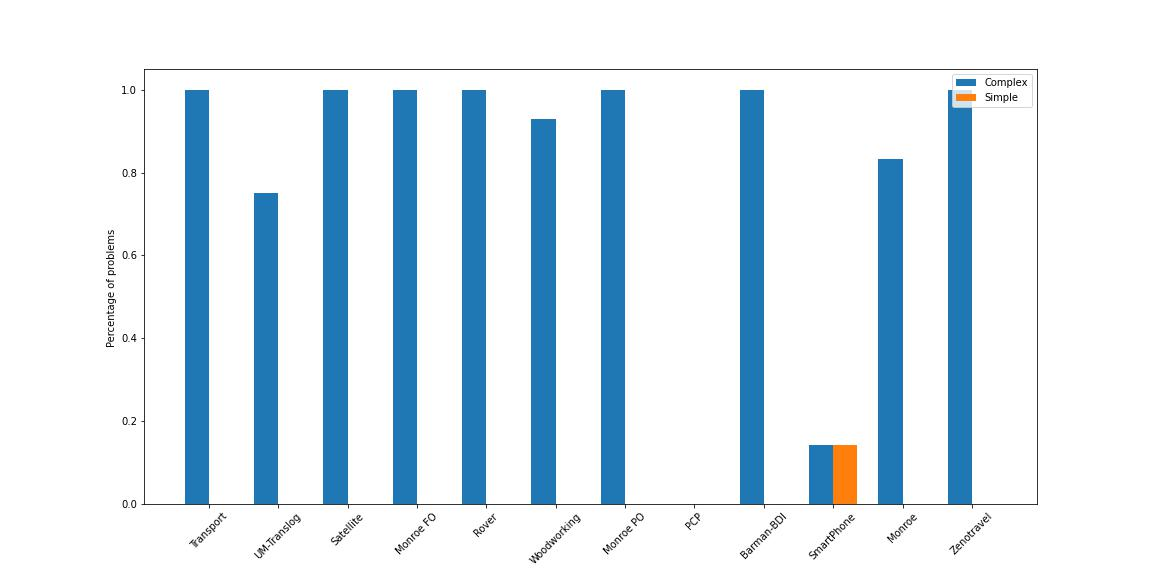
\includegraphics[width=14cm]{figures/Lin_criteria_C_vs_S.jpg}
%\end{figure*}


%\begin{figure*}
%	\caption{For Grounded Problems, Average Percentage of Methods Linearized Without %Cycle-break for Each Domain and for Each Inference Method}
%	\label{fig:MethodsLinearizedWOCycleBreak}
%	\centering
%	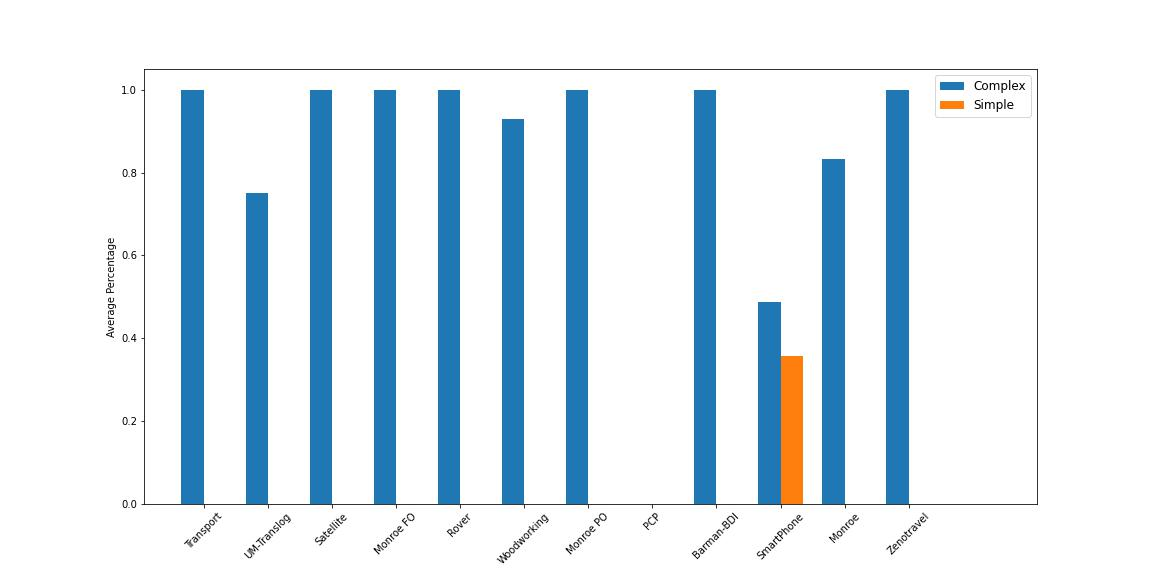
\includegraphics[width=14cm]{figures/Lin_average_C_vs_S.jpg}
%\end{figure*} 


\section{Related Work}
There exist other planners that also compile POHTN problems to decidable planning classes e.g. the planners by \cite{HTN2STRIPS} and HTN2SAS planner by \cite{HTN2SAS} convert POHTN to classical planning problems. To the best of my knowledge, this is the first work that focuses on converting POHTN to TOHTN problems.

\cite{ErolHTNExpressivity} proved that it is NP-complete to decide whether a partially ordered set
of actions has an executable linearization. Our criteria would work on a problem where the only method is for the initial task, and it’s sub-tasks are actions. That is essentially just ordering a partially ordered plan, so the criteria can also identify a proper subset of all partially ordered plans that can be linearized in polynomial time. It can also find a executable linearization for that subset in polynomial time.


\cite{NEBEL1994125} studied various questions regarding partially ordered plans, such as the complexity of plan existence, plan optimisation, possible or necessary truth of properties before or after plan steps, given various constraints on the types of tasks allowed.  \cite{KambhampatiModalTruth1996} studied related questions and criteria under different assumptions.
In the paper by \cite{TanGruningerPOPlanComplexity}, the authors refine \cite{NEBEL1994125}'s results and show the impact of the interaction of preconditions and effects thereby giving a more detailed picture for when finding a linearization for a partially-ordered plan is possible in polynomial time, and when it remains NP-hard. 

Criteria presented in \cite{NEBEL1994125} and \cite{KambhampatiModalTruth1996} and  \cite{TanGruningerPOPlanComplexity} analyse cases where actions have singleton precondition and add lists. This is a less general case than our criteria can cover, but their criteria also correctly identifies some cases as linearizable in polynomial time that our criteria is unable to determine. Thus their results are orthogonal to ours. 

The paper by \citet{DeleteRelaxation, Bercher2021POCLComplexities} generalised \cite{NEBEL1994125}'s as well as \cite{ErolHTNExpressivity}'s result (deciding whether a partially ordered
set of actions possesses an executable linearization) by showing that this problem does not become easier when one is allowed to insert delete-relaxed  actions.

\section{Future Work}
%Encode Linearization Problem as a MAX-SAT Problem
The maximum satisfiability problem (MAX-SAT) is the problem of determining the maximum number of clauses, of a given Boolean formula in conjunctive normal form, that can be made true by an assignment of truth values to the variables of the formula. MAX-SAT is used over SAT as it may not be possible to satisfy all orderings implied by the inferred preconditions and effects.

The current linearization procedure considers each method in isolation, and sub-tasks have their inferred $\PreS, \AddS, \DelS$. Thus we can treat each sub-task as a \enquote{action}, and encode the method the same way as a classical plan, as described by \cite{RINTANEN201245}, but with the additional constraint that \enquote{actions} chosen from the method sub-tasks can only be selected once, unlike in the domain.
% Assuming no negative preconditions, the initial state has all state variables true, and goal state can be assumed to be empty (i.e.\ all state variables can have any assignment). The relative success (or failure) of this approach could also lend insight into what about the criteria causes the linearization to be successful.


%Adding a Plan as Additional Input to the Domain
%Adding a plan as additional input to the PO domain having the semantics that this plan shall be in the solution set of the TO output model. This reduces the computational complexity of the decision problem from undecidable.  % I assume the resulting problem is PSPACE-complete, but this needs to be proven





\section{Conclusion}

% The contributions of this paper are as follows:

This paper finds that, at least for the POHTN problems in the IPC domain, most of them are not undecidable. In other words, it is as if the POHTN domains are compressed TO domains - this linearization separates one of them back out.

We can also see this pre-processing technique leads to large gains in time/efficiency for a number of planners, at least for the problems tested here. Furthermore, there is demonstrably much more room for improvement. Though the criteria does not fire all the time, it's producing a linearization that is almost always solvable.

This method can also be used to increase the number of TOHTN problems available for purposes like comparing TOHTN planners or grounding techniques. Suppose there were $n$ POHTN problms and $m$ TOHTN problems, and this linearization could make those $n$ POHTN problems into $k$ solvable $TOHTN$ problems. Then $k+m$ (lifted or grounded) TOHTN problems exist now. And from empirical evaluation, $k$ may be close to $n$.

Finally, in this paper we identify a subset of decidable problems within POHTN problems, and this subset is orthogonal to all others discussed in other works.









% Use \bibliography{yourbibfile} instead or the References section will not appear in your paper
\bibliography{bib}
% \nobibliography{aaai22}

\end{document}
